% !TeX spellcheck = en_US
\documentclass[winfonts]{njuthesis}
\usepackage{makecell}
%%%%%%%%%%%%%%%%%%%%%%%%%%%%%%%%%%%%%%%%%%%%%%%%%%%%%%%%%%%%%%%%%%%%%%%%%%%%%%%
% 设置论文的中文封面
% 论文标题
\title{基于超声波和IMU的室内定位系统}
% 论文作者姓名
\author{陈勇虎}
% 论文作者学号
\studentid{161240005}
% 导师姓名职称
\supervisor{谢磊}
% 导师职称
\supervisortitle{副教授}
% 论文作者院系
\department{匡亚明学院}
% 论文作者专业方向
\major{计算机科学与技术}
% 论文作者的年级
\grade{2016级}
% 论文提交日期,需设置年、月、日。此属性可选,默认值为最后一次编译时的日期,精确到日。
\submitdate{2020年5月20日}

%%%%%%%%%%%%%%%%%%%%%%%%%%%%%%%%%%%%%%%%%%%%%%%%%%%%%%%%%%%%%%%%%%%%%%%%%%%%%%%
% 设置论文的英文封面
% 论文的英文标题
\englishtitle{IMU}
% 论文作者姓名的拼音
\englishauthor{Yonghu Chen}
% 导师姓名职称的英文
\englishsupervisor{Professor Lei Xie}
% 论文作者所在院系的英文名称
\englishdepartment{School of Computer Science}
% 论文作者所在学校或机构的英文名称。此属性可选,默认值为``Nanjing University''。
\englishinstitute{Nanjing University}
% 论文完成日期的英文形式,默认最后一次编译的时间
\englishdate{May 20, 2020}
% 专业
\englishinstitute{Computer Science and Technology}

%%%%%%%%%%%%%%%%%%%%%%%%%%%%%%%%%%%%%%%%%%%%%%%%%%%%%%%%%%%%%%%%%%%%%%%%%%%%%%%
% 设置论文的页眉页脚
\usepackage{fancyhdr}
\pagestyle{fancy}
%\lhead{\bfseries 141180092 }
\chead{毕业论文}
\rhead{陈勇虎}
%\lfoot{From: K. Grant}
%\cfoot{To: Dean A. Smith}
%\rfoot{\thepage}
\renewcommand{\headrulewidth}{0.4pt}
%\renewcommand{\footrulewidth}{0.4pt}

%\makeatletter
%\newenvironment{breakablealgorithm}
%{% \begin{breakablealgorithm}
%	\begin{center}
%		\refstepcounter{algorithm}% New algorithm
%		\hrule height.8pt depth0pt \kern2pt% \@fs@pre for \@fs@ruled
%		\renewcommand{\caption}[2][\relax]{% Make a new \caption
%			{\raggedright\textbf{\ALG@name~\thealgorithm} ##2\par}%
%			\ifx\relax##1\relax % #1 is \relax
%			\addcontentsline{loa}{algorithm}{\protect\numberline{\thealgorithm}##2}%
%			\else % #1 is not \relax
%			\addcontentsline{loa}{algorithm}{\protect\numberline{\thealgorithm}##1}%
%			\fi
%			\kern2pt\hrule\kern2pt
%		}
%	}{% \end{breakablealgorithm}
%		\kern2pt\hrule\relax% \@fs@post for \@fs@ruled
%	\end{center}
%}
%\makeatother

\makeatletter
\newenvironment{breakablealgorithm}
{% \begin{breakablealgorithm}
	\begin{center}
		\refstepcounter{algorithm}% New algorithm
		\hrule height.8pt depth0pt \kern2pt% \@fs@pre for \@fs@ruled
		\renewcommand{\caption}[2][\relax]{% Make a new \caption
			{\raggedright\textbf{算法\thealgorithm} ##2\par}%
			\ifx\relax##1\relax % #1 is \relax
			\addcontentsline{loa}{algorithm}{\protect\numberline{\thealgorithm}##2}%
			\else % #1 is not \relax
			\addcontentsline{loa}{algorithm}{\protect\numberline{\thealgorithm}##1}%
			\fi
			\kern2pt\hrule\kern2pt
		}
	}{% \end{breakablealgorithm}
		\kern2pt\hrule\relax% \@fs@post for \@fs@ruled
	\end{center}
}
\makeatother

%%%%%%%%%%%%%%%%%%%%%%%%%%%%%%%%%%%%%%%%%%%%%%%%%%%%%%%%%%%%%%%%%%%%%%%%%%%%%%%
\begin{document}
% 制作中文封面
\maketitle
% 制作英文封面
% \makeenglishtitle
% 毕业论文过程管理四页表
\controlpage %可以将word文件交给老师签字后扫描转成pdf,然后命名为controlpage.pdf

% 论文的中文摘要
\begin{abstract}


基于IMU和智能手机的室内定位系统

% 同时应该注意到,空白页是故意留白,以便章节开头能够出现在偶数页。
% 中文关键词。关键词之间用中文全角分号隔开,末尾无标点符号。
\keywords{IMU; 智能手机; }
\end{abstract}

%%%%%%%%%%%%%%%%%%%%%%%%%%%%%%%%%%%%%%%%%%%%%%%%%%%%%%%%%%%%%%%%%%%%%%%%%%%%%%%
% 论文的英文摘要
\begin{englishabstract}
IMU
% 英文关键词。关键词之间用英文半角逗号隔开,末尾无符号。
\englishkeywords{IMU, smart phone, }
\end{englishabstract}

%%%%%%%%%%%%%%%%%%%%%%%%%%%%%%%%%%%%%%%%%%%%%%%%%%%%%%%%%%%%%%%%%%%%%%%%%%%%%%%
% 论文的前言,应放在目录之前,中英文摘要之后
%
%\begin{preface}
%
%在过去的40年中,手写中文文本领域识别(HCTR)取得了很大的进展[1,2]。
%
%\vspace{1cm}
%\begin{flushright}
%饶安逸\\
%2018年5月15日于南大仙林
%\end{flushright}
%
%\end{preface}

%%%%%%%%%%%%%%%%%%%%%%%%%%%%%%%%%%%%%%%%%%%%%%%%%%%%%%%%%%%%%%%%%%%%%%%%%%%%%%%
% 生成论文目录
\tableofcontents

%%%%%%%%%%%%%%%%%%%%%%%%%%%%%%%%%%%%%%%%%%%%%%%%%%%%%%%%%%%%%%%%%%%%%%%%%%%%%%%
% 生成插图清单。如无需插图清单则可注释掉下述语句。
%\listoffigures

%%%%%%%%%%%%%%%%%%%%%%%%%%%%%%%%%%%%%%%%%%%%%%%%%%%%%%%%%%%%%%%%%%%%%%%%%%%%%%%
% 生成附表清单。如无需附表清单则可注释掉下述语句。
%\listoftables

%%%%%%%%%%%%%%%%%%%%%%%%%%%%%%%%%%%%%%%%%%%%%%%%%%%%%%%%%%%%%%%%%%%%%%%%%%%%%%%
% 开始正文部分
\mainmatter

%%%%%%%%%%%%%%%%%%%%%%%%%%%%%%%%%%%%%%%%%%%%%%%%%%%%%%%%%%%%%%%%%%%%%%%%%%%%%%%
% 学位论文的正文应以《绪论》作为第一章
\chapter{绪论}\label{chapter_introduction}
	\section{研究背景及意义}
		在室内环境(办公室,住所)中想要寻找一个小物品,诸如钥匙,硬币,可以说是一件令人费神的事情了\cite{HyperEarAbstract}。在游戏世界和虚幻的电影场景中,我们都或多或少接触过类似于“寻宝罗盘”的神奇宝物,它可以类似一个掌上的指南针,时刻指示“宝物”的方向。随着各式各样移动智能设备的广泛涌现,例如智能手机,智能手表,这些设备不仅自带了诸多传感器,同时可以为用户提供很好的UI界面。因此,如果可以利用这些设备实现类似于寻宝罗盘的功能,用于寻找我们室内环境中的小物品,无疑是有趣且富有创造性的。
		
		随着对位置精度要求的提高,对于定位技术的研究也越加深入。传统的全球定位系统(Global Positioning System,GPS)\cite{wikipedia_GPS}是现代定位系统的首选,然而,在室内环境中,由于卫星信号受到建筑物的削弱,遮蔽,以及在复杂的室内环境下引起的信号反射,折射,透射等造成的多径和非视距传输现象, 导致定位误差较大,所以卫星定位的精度已经无法满足室内定位的需求,因此以无线传感网为媒介的定位系统逐渐发展起来。
		
		
	
	\section{国内外研究现状}


	\section{研究内容与本文主要工作}

		\begin{enumerate}
		\item
			
		\item
			
		\item 
			
		\end{enumerate}

	\section{本文的整体结构}
		本文共分为个章节,每个章节具体安排如下:
		
		第一章 绪论。
		 
		第二章 相关工作
		
		第三章 实验
		
		第四章 总结与讨论
		
		。。。

%%%%%%%%%%%%%%%%%%%%%%%%%%%%%%%%%%%%%%%%%%%%%%%%%%%%%%%%%%%%%%%%%%%%%%%%%%%%%%%
\chapter{声源定位相关研究工作}
	\section{声源定位技术介绍}
		
		噪声和异响是日常生活和工业生产中所常见的现象,在很多情况下,这些声音是令人困扰的。至于如何去解决这些噪声,我们首先需要去识别噪声并且能够定位出噪声的方向和位置,这就是声源定位问题的一个实例。当然,声源定位技术并不局限于噪声的定位,在特定的场合中,也有不同的应用。例如在会议室中,定位正在说话人的位置同样是声源定位技术的应用。
		
		日常生活中我们似乎很容易根据听到的声音来辨别声源的大致方向,比如从身边急驶而过的汽车的来向,甚至车辆距离自己大概的距离。经过专业的训练,我们甚至可以让盲人参与到踢足球的运动中。这种常见的“听声辨位”尽管有一定的局限性,但是依然可以满足我们生活中很多的定位需求。借助于双耳效应的启发,为了提高声源定位的分辨力,声源定位技术提出了很多高效的定位方案。本章将对声源定位方案,双麦系统等进行调研。
		
	\section{声源定位方案}
	
		在现代城市中,利用机器视觉实现的机器人导航系统已是非常普遍。然而由于机器视觉本身存在的问题,使得利用机器视觉进行机器人导航在一些环境下表现的差强人意,比如,在光线不足的情况下,或者是在机器人的“视野”所不能到达的地方,机器人就找不到目标在空间中的位置,如果给机器人安装上“耳朵”,给予机器人声源采集装置,在进行人机交互的时候,人就可以通过语音告诉机器人自己现在所处的位置,机器人对声源信号进行处理,求解出声源的具体位置,然后制定关节运动决策,使交互对象重新进入其视野之内。
		

%%%%%%%%%%%%%%%%%%%%%%%%%%%%%%%%%%%%%%%%%%%%%%%%%%%%%%%%%%%%%%%%%%%%%%%%%%%%%%%	
\chapter{智能手机感知与定位原理}\label{chapter_mobile}
	
	近些年来,基于声学传感器的定位系统越来越受到人们的关注,依赖于多个同步的麦克风,采集到的多路同步信号,用以后续的信号处理。随着无线传感网的不断发展进步,无线传感网定位问题也是一个比较热门的课题。而节点定位作为目标定位的前提条件,节点的定位精度也影响着目标定位的结果。然而,尽管目前有很多节点定位算法,但是因为功耗,成本等客观条件的限制,这些定位算法在很多场景中并不能很好的应用。因此本文提出了一种可以在室内环境下利用智能手机进行定位的方案。
	
	随着智能设备的普及以及诸多传感器的集成,智能手机与硬件技术的协同发展有目共睹。无论是ios系统还是Android系统下的智能手机,内置传感器也越加丰富,也为智能手机应用的发展带来了更多的可能。

	本文将会对利用智能手机进行双麦结点定位进行简要描述,并对本文中后续所涉及的智能手机内置传感器进行讲解,最后系统描述本文中所使用的的一些定位原理和算法设计。

	\section{双麦克风的节点定位}
	
	随着可移动智能设备的普及,尤以智能手机更为常见。自2018年起,大部分的智能手机都开始集成两个甚至多个麦克风,除了底部的通话话筒以外,智能手机的顶部都还有一个“小孔”(不同的手机可能有所区别,例如iPhone手机的次麦克风可能位于主摄像头的附近)(如图\ref{fig: iphone-dual-microphone}),这就是手机的降噪麦克风,它的主要作用是实现有噪声环境下的高质量通话。
	
	\begin{figure}[htbp]
		\centering
		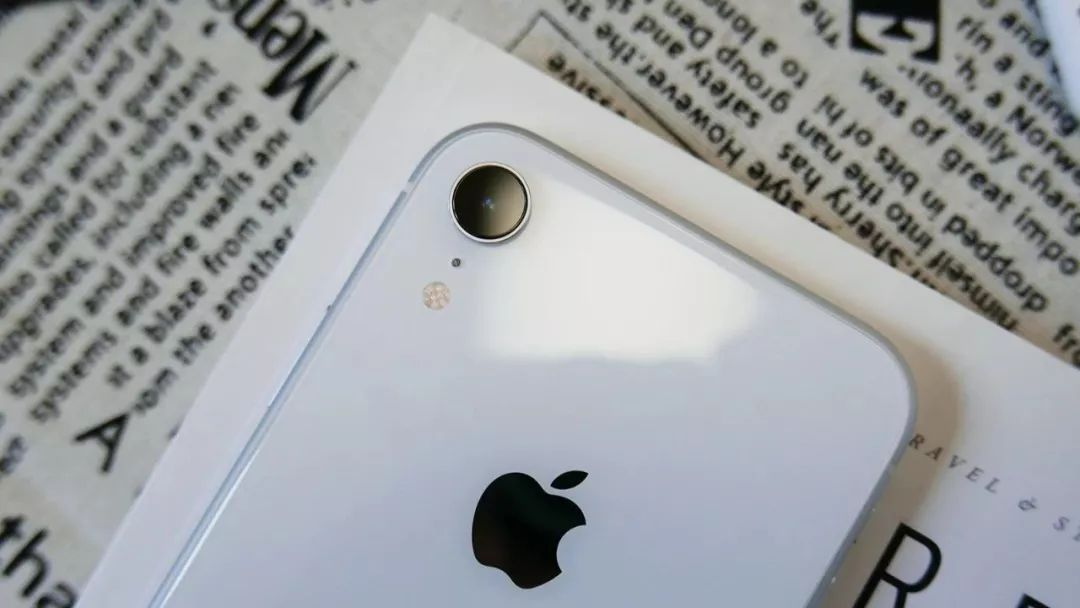
\includegraphics[width=0.7\textwidth]{iPhone-dual-micphone.jpeg} 
		\caption{iPhone8的次麦克风手机位于摄像头附近}
		\label{fig: iphone-dual-microphone}
		%\vspace{0.8cm} % 用来调整和下方文字的间距
	\end{figure}
	
	手机上设有的两个电容式麦克风尽管作用不同,但是其性能相同,对声音信号的收集能力相同。利用双麦克风系统的时间同步(两个麦克风是集成于同一个设备的,因此完全时钟同步)特性,即使两个麦克风(如图\ref{fig: samsung-dual-microphone})之间的距离较短(16cm左右,不同手机略有差异),也可以根据声音到达两个麦克风时刻的差异计算TDOA,因此,利用双麦克风系统手机结点作为实验设备有效解决了研究过程中时钟同步的问题。
	
	\begin{figure}[htbp]
		\centering
		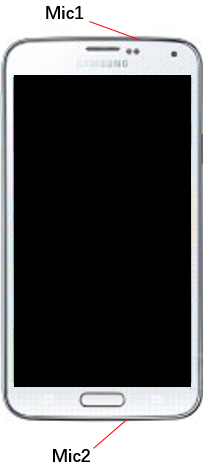
\includegraphics[height=0.35\textheight,width=0.3\textwidth]{samsung-dual-microphone.png} 
		\caption{Dual-microphone phone}
		\label{fig: samsung-dual-microphone}
		%\vspace{0.8cm} % 用来调整和下方文字的间距
	\end{figure}
	
	目前已经有很多利用双麦克风结点实现声源定位或者其他有趣的研究成果。例如利用双麦克风智能手机进行手势轨迹感知\cite{VSkin};Aarab 使用双麦克风节点定位的思路测算说话人的位置\cite{DMArrays}。
	
	\section{智能手机的传感器}
	
	随着技术的进步,手机已经不再是一个简单的通信工具,而是具有综合功能的便携式电子设备。大多数的ios和Android设备都有许多内置传感器,用来测量运动,屏幕方向和各种环境条件,这些传感器能够提供高度精度的原始数据,非常适合用来测量设备的三维移动和定位,或者检测设备周围环境的变化,例如可以跟踪设备的重力传感器推断用户的手势和动作,同样天气应用中将会使用设备的温度传感器和湿度传感器。智能手机的内置传感器有硬件实现和软件实现之分\cite{Google_Sensor}。基于硬件的传感器是内置在手机或者平板设备中的物理组件,这类传感器通过直接测量待定的环境属性(如加速度,地磁场强度或者角度变化等)来采集数据。基于软件的传感器不是物理设备,从一个或者多个硬件传感器获取数据,例如线性加速度传感器。具体可参考表\ref{table: Android Sensor}。本章将会简述实验中涉及使用的几种传感器。
	
	\begin{table}[htbp]
		\caption{Android 平台支持的传感器类型}
		\centering
		\begin{tabular}{cccc}
			\hline 
			传感器	& 类型 & 说明 & 常见用途\\
			\hline
			\text{ACCELEROMETER} & 硬件 & 加速力 & 动态检测\\
			\text{AMBIENT\_TEMPERATURE} & 硬件 & 环境室温 & 监测气温\\
			\text{GRAVITY} & 软件或硬件 & 重力 & 动态检测 \\
			\text{GYROSCOPE} & 硬件 & 旋转速率 & 旋转检测 \\
			\text{LIGHT} & 硬件 & 环境光级(照度 & 控制屏幕亮度 \\
			\text{LINEAR\_ACCELERATION} & 软件 & 加速力 & 监测单个轴向上的加速度\\
			\text{MAGNETIC\_FIELD} & 硬件 & 环境地磁场 & 创建罗盘 \\
			\text{ORIENTATION} & 软件 & 旋转角度 & 确定设备位置 \\
			\text{PRESSURE} & 硬件 & 环境气压 & 监测气压变化 \\
			\text{PROXIMITY} & 硬件 & 物体到屏幕的距离 & 通话过程中手机的位置 \\
			\text{RELATIVE\_HUMIDITY} & 硬件 & 环境的相对湿度 & 露点,绝对湿度和相对湿度 \\
			\text{ROTATION\_VECTOR} & 软件或硬件 & 设备 & 动态检测和旋转检测\\
			\text{TEMPERATURE} & 硬件 & 设备 & 监测温度 \\
			\hline
		\end{tabular} 
		\vspace{0.2cm}
		\label{table: Android Sensor}
	\end{table}
	
		\subsection{加速度传感器}
			
		
		\subsection{陀螺仪}
		
		\subsection{重力传感器}
		
		\subsection{磁力计}
	
	\section{到达时间差(TDOA)}
	
	\section{基于到达时间差的定位算法设计}
	
	\section{}
	
%%%%%%%%%%%%%%%%%%%%%%%%%%%%%%%%%%%%%%%%%%%%%%%%%%%%%%%%%%%%%%%%%%%%%%%%%%%%%%%
\chapter{基于双麦克风手机的声源定位方案}\label{chapter_work}
	近些年来,智能手机已经成为人们生活中不可缺少的一部分,手机上集成的传感器的发展,使得智能手机的功螚越来越强大。在前面我们已经简述到大部分智能手机已经配备两个麦克风,用于消除我们在日常通话中的环境噪声,并且可以很好的解决的时钟同步问题。因此,利用智能手机的优势,通过获取同一个手机两个麦克风的声音数据,我们从中过滤出我们想要的声音信号,得到两路同步的声音信号,利用智能手机计算出两个麦克风的到达时间差(TODA),对TDOA信号进行后续的处理,就可以实现一些有意义的功能。
	
	在前一章的基础上,本章详细描述利用双麦克风手机实现定位功能的诸多细节性工作。
	
	\section{离线数据处理流程}
	
		本小节中,首先介绍offline算法的处理流程,并逐渐过渡到最终系统使用的online算法的处理流程。offline算法中,智能手机会收集声音文件并产生一个wav文件,通过MATLAB分析该wav文件,计算出TDOA。该offline算法处理流程是为了通过处理一段时间窗口内,设备没有发生大幅度状态变化(包括角度,位置等参数)的情况下,计算出静态声源相对于该位置的方向(Speaker Direction Finding (SDF))。在一段时间窗口内的处理流程如下图所示(\ref{fig: offline-flowchart}).
		
		\begin{figure}[H]
			\centering
			\caption{offline flowchart}
			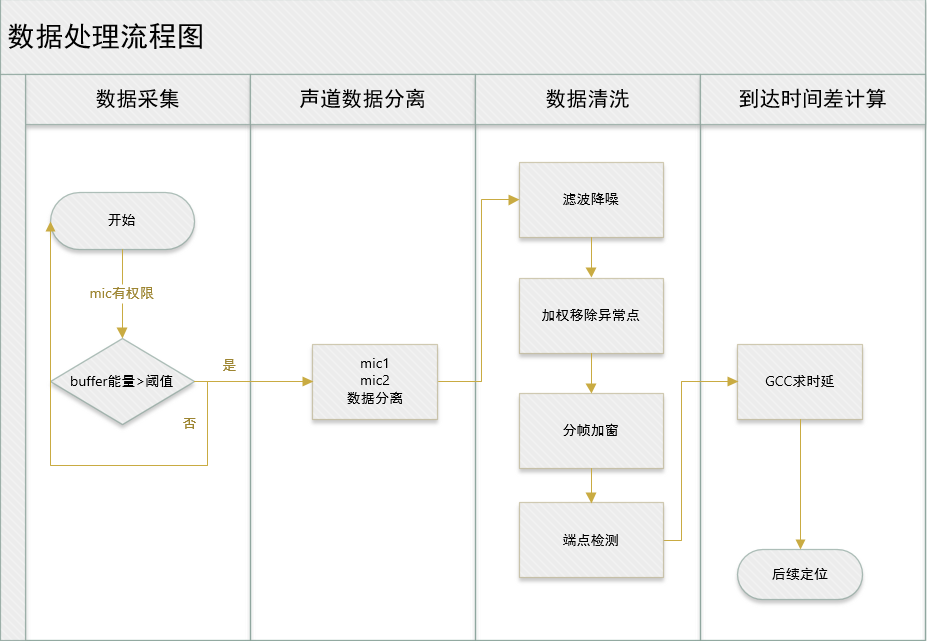
\includegraphics[scale = 0.5]{offline-flowchart.png} 
			\label{fig: offline-flowchart}
			%\vspace{0.8cm} % 用来调整和下方文字的间距
		\end{figure}
	
	\section{数据采集}
		本文利用具有双麦克风系统的智能手机(Samsung 5)作为传感器结点的进行声音信号的手机,在分析阶段,使用MATLAB科学工具对采集到的信号进行解析显示。我们利用另一台手机发出了一个频率在2000Hz-2700Hz变换的线性调频信号,如图\ref{fig: dual-microphone-data}所示,图中蓝色的标记为LY的数据以及红色的标记为RY的数据,分别代指两个麦克风采集的数据。图中的上一部分图中,横坐标代指数据采样点,纵坐标是对数据进行标准化后的结果,因此无量纲。但是在下部分图中,横坐标是标准化的频率,单位为$\pi * $radians/sample(频率标准化的相关概念不做赘述,可以参考\cite{Normalized_frequency}),纵坐标为能量谱,这里我们很容易看出两个麦克风的采集的数据的能量谱是非常接近的,换句话说,两个麦克风的采集能力非常接近。这里我们对原始数据取样其中发生部分连续的400个点。如图\ref{fig: dual-microphone-data1}所示,同样我们依然可以看出两个麦克风的采集能力是非常接近的,另一方面,即便我们暂时无法确定TDOA的值,但是我们可以清晰看出两路声音数据是差了几个样本点的,因此只要计算出相差的样本点数,根据采样率(44100Hz)我们就可以求解出TDOA的近似的结果。
		
		\begin{figure}[H]
			\centering
			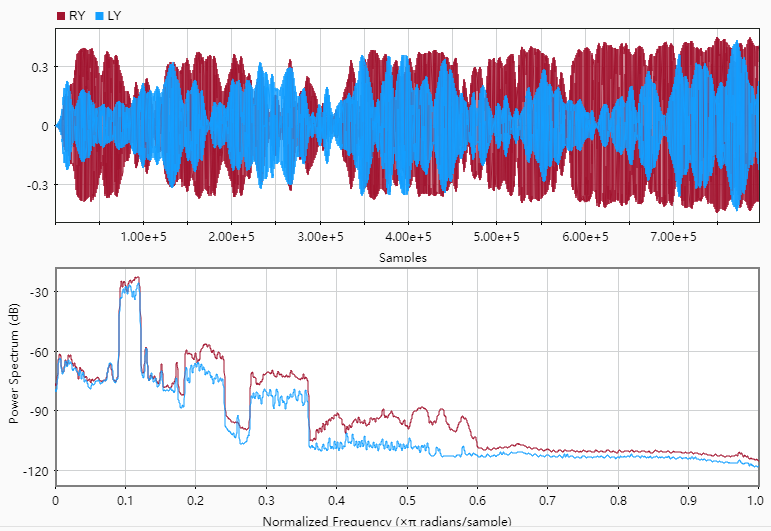
\includegraphics[width=\textwidth]{dual-microphone-data.png} 
			\caption{双麦克风信号}
			\label{fig: dual-microphone-data}
			%\vspace{0.8cm} % 用来调整和下方文字的间距
		\end{figure}
	
		\begin{figure}[H]
			\centering
			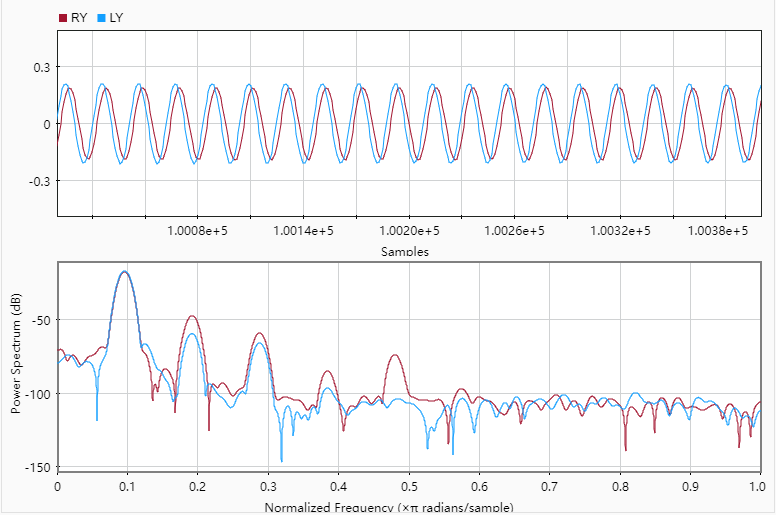
\includegraphics[width=\textwidth]{dual-microphone-data1.png} 
			\caption{双麦克风信号取样}
			\label{fig: dual-microphone-data1}
			%\vspace{0.8cm} % 用来调整和下方文字的间距
		\end{figure}
		
		下表中\ref{table: parameters-of-S5}展示了采集声音信号的手机参数,实验中使用了SamSung S5手机作为实验设备,S5集成了两个同步的麦克风,分别位于手机的底部和顶部,而这个两个麦克风的声音采集能力完全相同。目前的智能手机最高采样率都可以达到44100Hz,每秒钟就可以获得44100个声音信号的样本值。
		
		\begin{table}[htbp]
			\setlength{\belowcaptionskip}{7pt}
			\caption{SamSung S5设备参数}
			\centering
			\begin{tabular}{ccc}
				\hline 
				参数 & 描述 \\
				\hline
				灵敏度 & -26dB\\
				麦克风距离 & 16cm \\
				采样频率 & 44100Hz\\
				\hline
			\end{tabular} 
			\vspace{0.2cm}
			\label{table: parameters-of-S5}
		\end{table}
	
		本文利用内置双麦克风的S5手机进行实时采集声音信号,首先介绍offline处理的,对信号进行汇总处理和分析。在底层获取的声音信号实际是个一维数组,当然利用MATLAB进行读取,会转换成两个一维数组,分别代表两个麦克风的数据。在原始的底层存储中,一维数组的值即是采集的到数据。如图\ref{fig: sound-data}所示,实验中,我们采用16bit的stero的格式进行采集,因此根据图中的存储方式很容易分别获得两个麦克风的数据,并且两组数据是完全满足时钟同步的。为了环境噪声或者其他声音的干扰,本文中设置了一个基于能量的硬阈值,当每个buffer信号的能量低于该阈值时,则认为没有声源发生,当平均能量高于该阈值时,认为有声源发生,从而进行后面的处理。
		
		\begin{figure}[H]
			\centering
			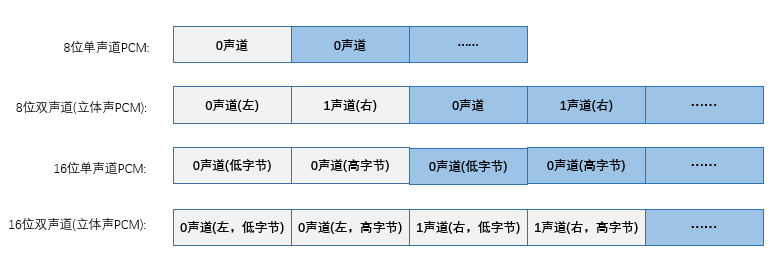
\includegraphics[scale=0.6]{sound-data.png} 
			\caption{数据存储方式}
			\label{fig: sound-data}
			%\vspace{0.8cm} % 用来调整和下方文字的间距
		\end{figure}
		
		数据采集阶段核心代码如果\ref{alg: data-collecting}所示.手机调用麦克风不断检测周围环境的声音信号,当信号端的平均能量高于阈值时,系统判断声源发声,并且将两路的声音信号进行分离,用于后续的处理。
		
		\begin{breakablealgorithm}
			\caption{dual-microphone signals acquisition(双麦克风信号采集)}
			\label{alg: data-collecting}
			\begin{algorithmic}[1]
				\STATE {mAudioRecord.startRecording()}
				\STATE {//系统检测周围环境中的声音信号} 
				\WHILE{isRecording}
					\STATE {//读取两路声音信号} 
					\STATE {read = mAudioRecord.read(mBuffer, 0, BUFFER\_SIZE)}
					\IF {read <= 0}
						\STATE {return false}
					\ELSE
						\STATE {//根据设定的阈值判断是否有声源发声}
						\STATE { sum = 0}
						\FOR{$i=0$ to read} 
							\STATE {sum += Math.abs(mBbuffer[i])}
						\ENDFOR 
						\STATE {//达到设定的阈值,认为有声源发声}
						\IF{sum / read > thresholdValue}
							\STATE {//两路信号分离}
							\STATE {index = 0}
							\FOR{$i=0$ to mBuffer.length/2}
								\IF{i \% 2 == 0}
									\STATE{System.arraycopy(mBuffer, i * 2, mBuffer1, 0, 2)}
									\STATE{LY[index] = ((mBuffer1[0]\&0x000000FF) | (((int)mBuffer1[1])<<8))/ 32768.0}
									\STATE{LYList.add(LY[index])]}
									\STATE{index = i / 2}
								\ELSE
									\STATE{System.arraycopy(mBuffer, i * 2, mBuffer2, 0, 2)}
									\STATE{RY[index] = ((mBuffer2[0]\&0x000000FF) | (((int)mBuffer2[1])<<8))/ 32768.0}
									\STATE{RYList.add(RY[index])]}
								\ENDIF
							\ENDFOR
						\ENDIF	
						\STATE {//other code for further data-processing}			
					\ENDIF
				\ENDWHILE
			\end{algorithmic}
		\end{breakablealgorithm}
	
	\section{声音信号处理}
	
		从底层获得的两路原始信号包括了真实声源信号,环境噪声以及其他各种异常点,本小节将会利用滤波器降低环境噪声的影响,同时使用加窗移动的方式去除采集中的异常值,对原始的信号进行清洗处理。

		\subsection{信号除噪}
		
			常见的去噪方式就是使用滤波器,这里我们使用带通滤波器,降低环境噪声的干扰。在MATLAB通过filter,designfilter函数我们很容易实现我们需要的功能,在后续的online算法处理流程中,因为程序运行在Java平台上,所以Android方面使用dsp-collection这一个jar包即可满足我们需要的功能。
			
			例如当我们的声源频率范围在2000Hz-2700Hz时,那么在除噪的过程中,我们就需要通过一个带通滤波器,减益非该频率范围的成分。如图(\ref{fig: filter-data})所示,横纵坐标信息同图(\ref{fig:dual-microphone-data})通过滤波,不在制定频率范围的数据被大大减益,从而降低了对实验结果的影响。
			
			\begin{figure}[ht!]
				\centering
				\begin{subfigure}{.45\textwidth}
					\centering
					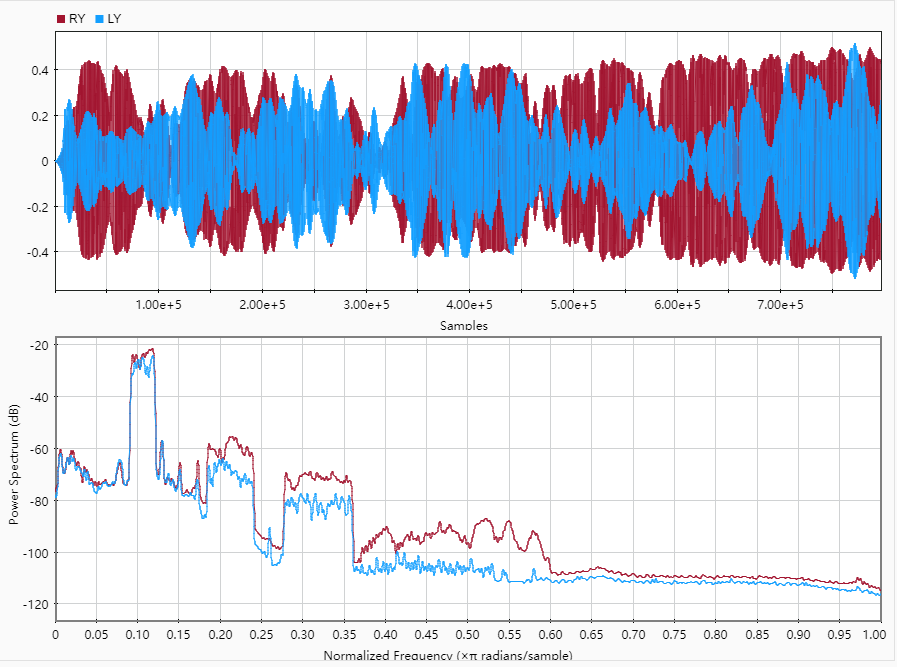
\includegraphics[width=0.9\textwidth]{data-unfiltered.png}
					\caption{信号除噪之前}
				\end{subfigure}
				\begin{subfigure}{.45\textwidth}
					\centering
					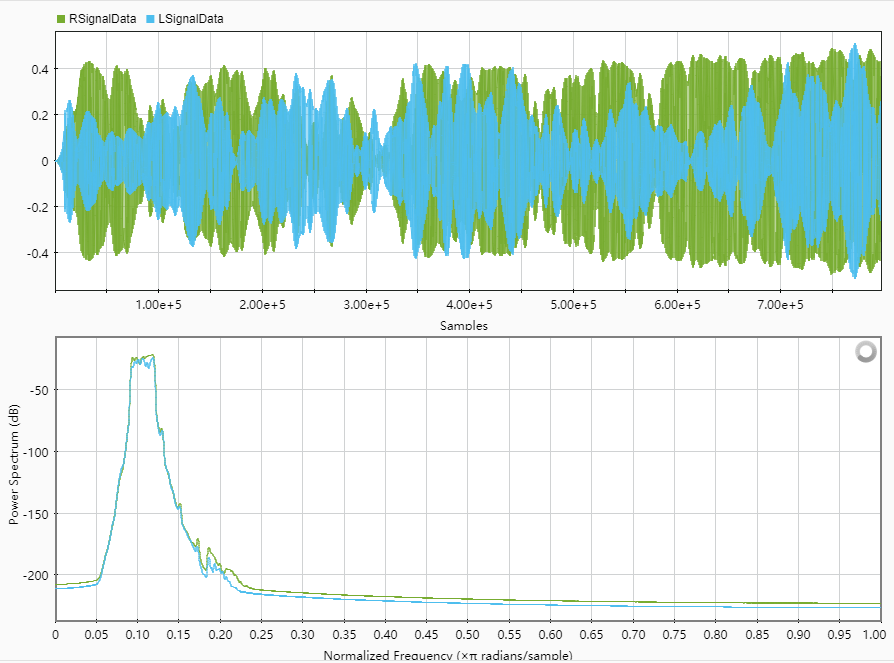
\includegraphics[width=0.9\textwidth]{data-filtered.png}
					\caption{信号除噪以后}
				\end{subfigure}
				\caption{(a)数据除噪之前。(b)数据除噪以后。}
				\label{fig: filter-data}
			\end{figure}
					
		\subsection{异常点移除}
		
			对实验结果影响较大的还有异常数据,例如在稳定的信号中仍会有一些突变的声音信号。为防止信号之间的干扰,这里采用分别对两路信号进行处理。值得一提的是,由于采样率高达44100Hz,所以处理过程中去掉一些数据并不会造成较大的影响。这里,我们采用滑动窗口的方式,使用加权平均移动(\text{WMA}\cite{Moving_average})的方式进行处理。加权平均移动认为:同一个窗口内的不同的数据对目标值都有着不相同的权重因子,因此目标值就可以看成窗口内数据和一个固定的权重函数的卷积。由于数据本身异常点并不是很多,并且使用传统的\text{WMA}就可以获得较好的效果,因此记$\text{signal}_t$为t时刻的数据,采用下面的公式更新t时刻的信号值:
			
			\begin{equation}
			\begin{aligned}
				\text{signal}_{t_{new}} = \text{WMA}_{t}&=\frac{n p_{t}+(n-1) p_{t-1}+\cdots+2 p_{(t-n+2)}+p_{(t-n+1)}}{n+(n-1)+\cdots+2+1}\\
											  &=\frac{n \times \text { signal }_{t-1}+(n-1) \times \text {signal}_{t-1}+\cdots+1 \times \text {signal}_{t-n+1}}{n+(n-1)+\cdots+2+1}								 
			\end{aligned}
			\end{equation}
			
			经过上述处理后,数据变得更加光滑,并且从图\ref{fig: data-outliers-removed}中已经可以隐约可见TDOA的大致范围。这里,\text{LSD}为第一个麦克风降噪后是数据,\text{LSignaData}代表降噪后数据经过异常点去除操作后的数据。
			
			\begin{figure}[H]
				\centering
				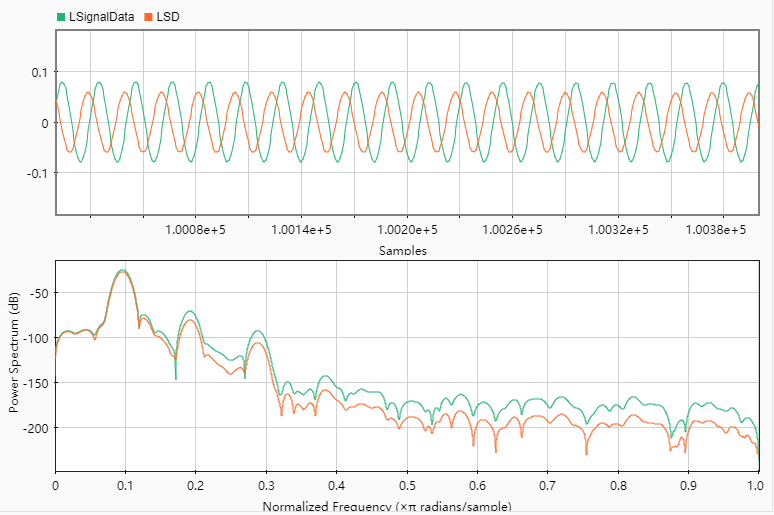
\includegraphics[width=\textwidth]{data-outliers-removed.png} 
				\caption{异常点移除后的数据}
				\label{fig: data-outliers-removed}
				%\vspace{0.8cm} % 用来调整和下方文字的间距
			\end{figure}
		
		\subsection{有效声音提取}
		
			阈值中值判断,online算法中去除 
		
			TODO
		
		\subsection{TDOA计算}
			
			本小节基于前期的信号处理获取到两路同步的声音信号,调用传统的GCC算法对两路同步信号进行TDOA计算(估计)。
			
			由于接收到的声音信号来自于同一个声源,因此两路信号之间具有较强的相关性而与噪声无关。广义互相关方法恰好可以得到两路信号之间的时延差。其基本思想是对两路信号$x_1(t)$和$x_2(t)$进行预滤波,然后再求互相关函数,其原理框架如图(\ref{fig: GCC})所示,公式表达为:
			
			\begin{equation}
				\tau_{\text {delay }}=\underset{t \in \mathbb{R}}{\arg \max }((f \star g)(t))
			\end{equation}
			
			\begin{figure}[H]
				\centering
				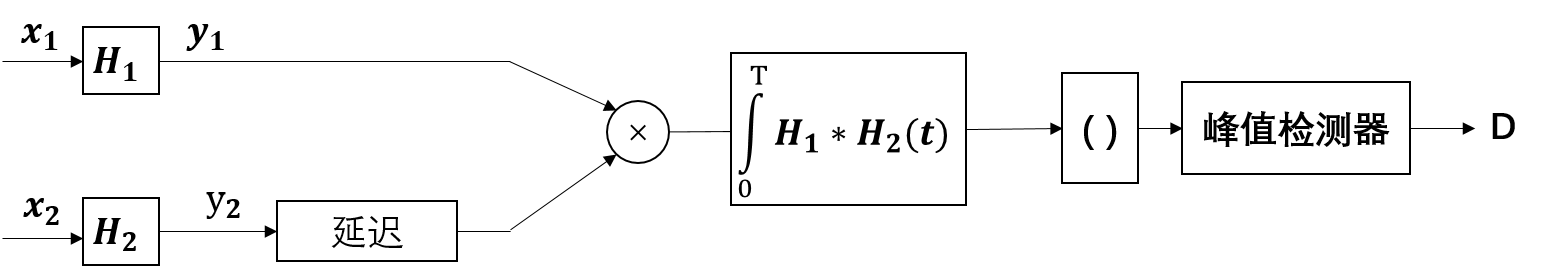
\includegraphics[width=\textwidth]{GCC.png} 
				\caption{Priciple diagram of the generalized cross-correlation based time delay estimation}
				\label{fig: GCC}
				%\vspace{0.8cm} % 用来调整和下方文字的间距
			\end{figure}	
			
			需要注意的是,这里计算出的“时延”实际是两个信号相差的采样点数,但是,由于采样率为设定好的44100Hz,因此计算出相差的采样点数,经过转换就可以得到对应的时延,也就是所求的TDOA,后面我们用相差的采样点数代指TDOA,转换公式无需赘述。可以明确的是,当TDOA < 0时,声音先到达第二个麦克风,TDOA > 0 时,声音先到达第一个麦克风,TDOA = 0 时,声音同时到达。降至二维空间下,详情如图(\ref{fig: tdoa})所示。
			
			\begin{figure}[H]
				\centering
				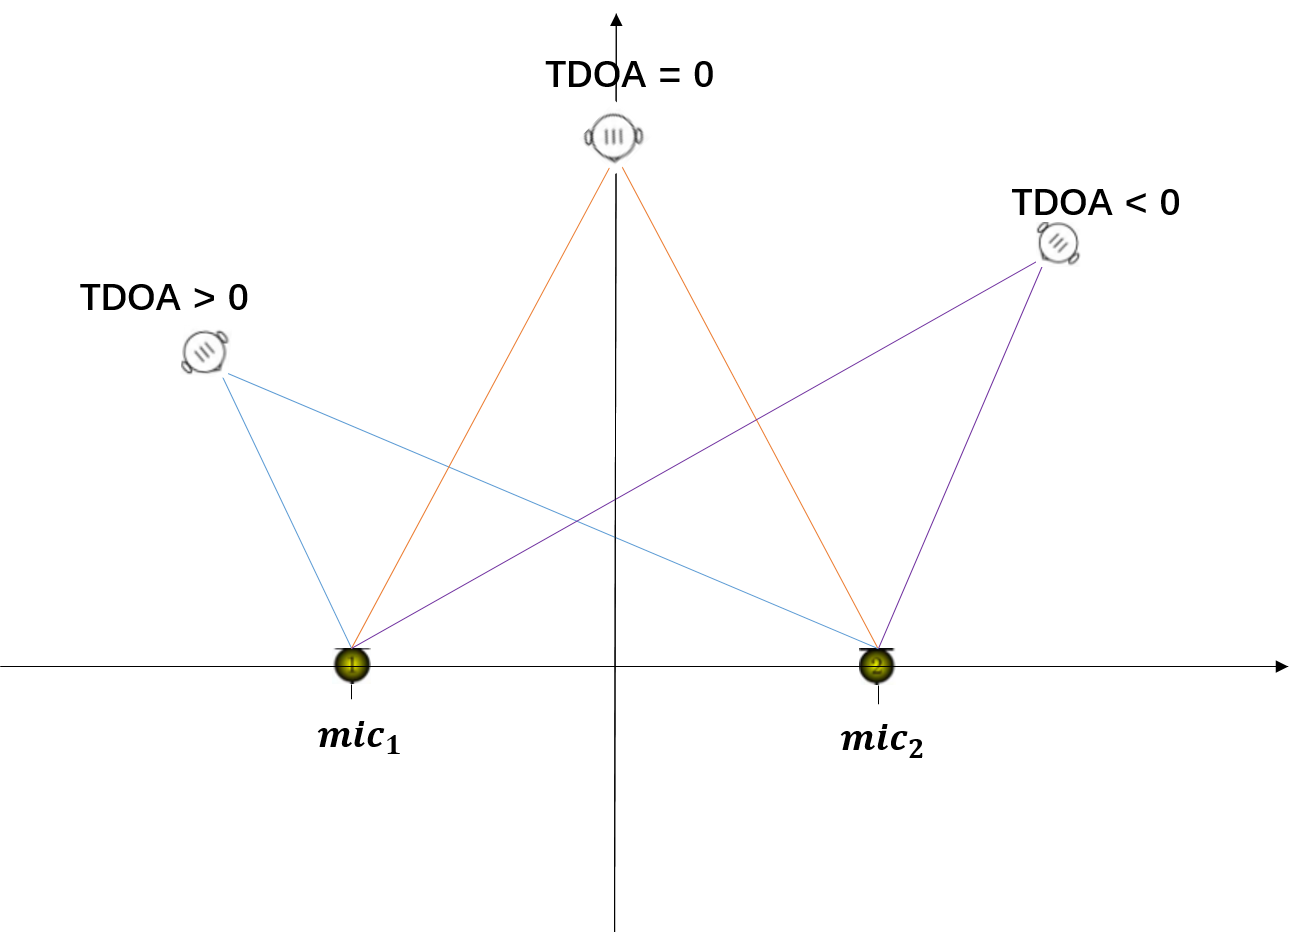
\includegraphics[width=\textwidth]{tdoa.png} 
				\caption{{\text{TDOA > 0, TDOA < 0, TDOA = 0}}}
				\label{fig: tdoa}
				%\vspace{0.8cm} % 用来调整和下方文字的间距
			\end{figure}
		
		\subsection{TDOA处理}
		
		利用智能手机作为传感器,计算指定声源到达同一个手机麦克风的TDOA,可以得到大量的数据并且计算出很多个数据段的TDOA。因此鉴于数据量多的优势,那么我们就可以利用此优势进行数据的筛选。即便我们的某些TDOA测量并不是足够“精确”,但是依然可以辅助进行方向探测。
		
		回到最初的系统设置,我们设置的采样率44100Hz,编码为16bit,我们暂时不考虑高编码编码的精确度,但显然的是,由于使用的bit数较大,因此数据量化的范围也更大,因此数据也是更精确的。对于44100Hz的采样率,麦克风每手机一秒钟,就可以采样到44100Hz的采样点。实验中发现,如果将太多量的数据一次性进行计算,由于我们没有加窗等操作,加上声源功率较小,信号衰减等,大部分测量结果都是不准确的。然而,另一方面,即便数据过多造成了结果不够准确,但是对数据分段,对该一秒钟的部分数据进行tdoa计算,在原理上也是对整段数据的tdoa的估计,因为延迟是“全局”的延迟,通过实验我们也发现这一个问题。因此,鉴于这种思想,我们可以将信号进行分段,当然,由于在后续实验中设备会一直处理数据,因此我们并不是对1s数据分段,而是每k个连续数据进行分段。从而,对两个麦克风相同次序的数据段进行TDOA,依然可以得到全局的TDOA,如图(\ref{fig: data-split})。
		
		\begin{figure}[H]
			\centering
			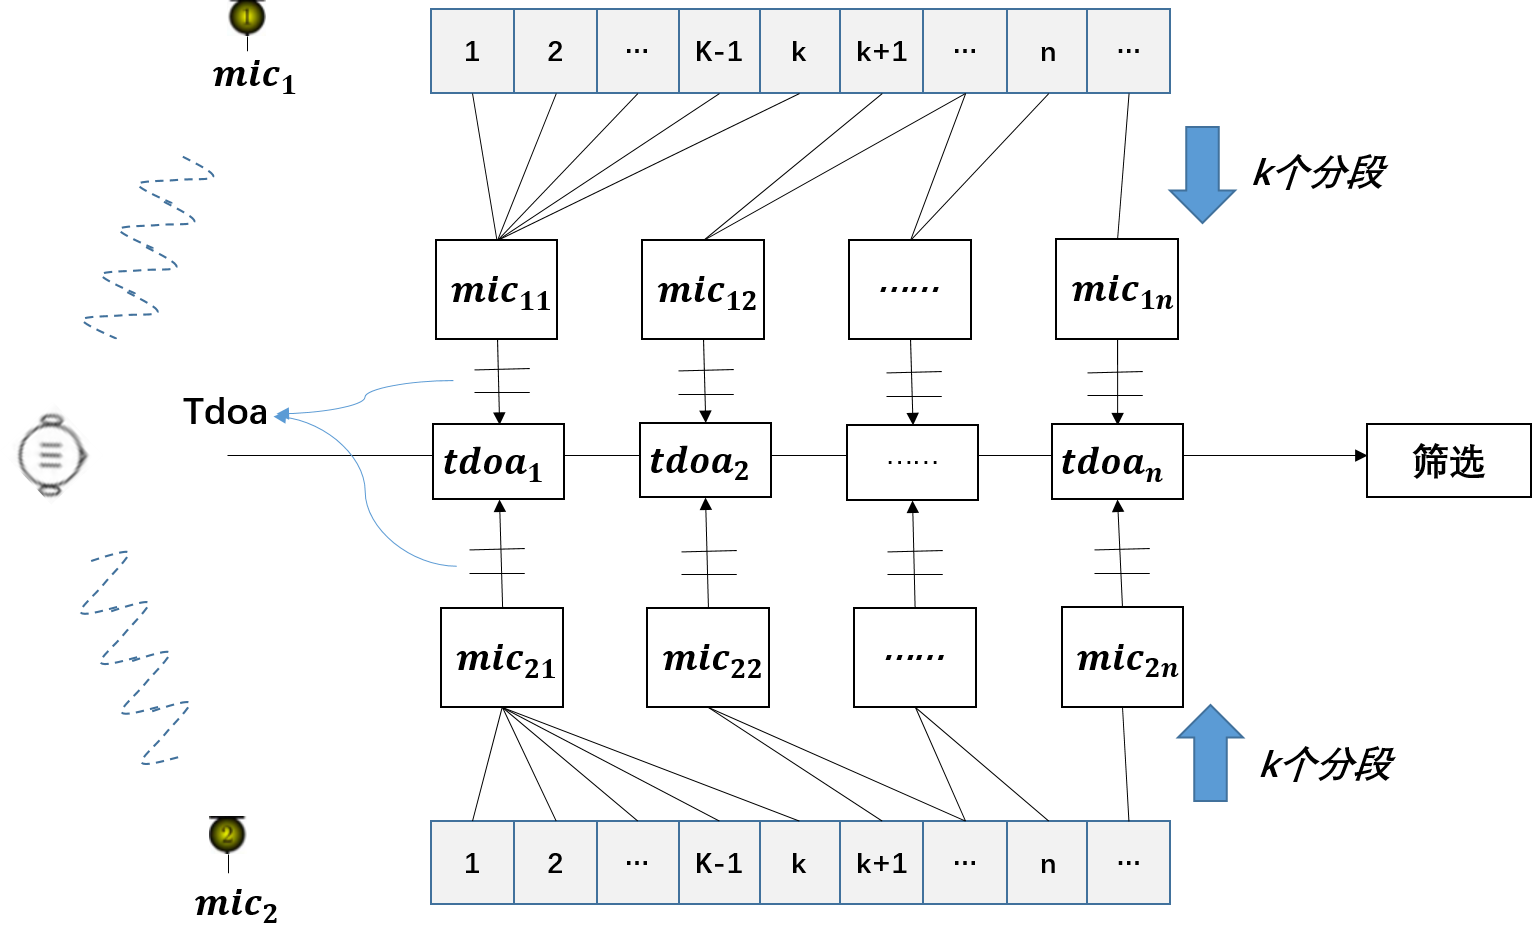
\includegraphics[width=\textwidth]{data-split.png} 
			\caption{{数据分段示意}}
			\label{fig: data-split}
			%\vspace{0.8cm} % 用来调整和下方文字的间距
		\end{figure}
		
		数据分段之后,并进行对应的数据段的tdoa计算,从而可以产生一系列的tdoa值。在实际计算中,我们设定k = 2048,很明显的是,对k的设定是一个trade-off的问题,若k值太小,数据点太少,基本无法得到合理的tdoa值,如果k值较大,精度会有影响,同时,也就没有分段的意义了,实验中k暂取用2048。另一方面需要明确的时,实验中手机麦克风距离约为16cm,因此tdoa绝对值的最大值$|\text{Tdoa}_{\text{max}}|$应该满足下式:
		
		\begin{equation}
			|\text{Tdoa}_{\text{max}}| = 16 / v * 44100 \leq 16 / 33700 * 44100  \approx 20.9 < 21
		\end{equation}
		
		因此Tdoa的范围应该在-21至21之间,这就是TDOA合理值的区间。另一方面,虽然由于离散采样的问题,Tdoa的值最后应该取整数,但是我们也可以肯定的是,即便有0.5个采样点的误差,$\delta distance = 0.5 / 44100 * v \leq 0.5 / 44100 * 34000 \approx 0.38cm$,对于16cm的麦克风距离来说,这个值微不足道。
		
		前面中我们提及到,部分信号计算的tdoa应该符合或者接近于全局的tdoa值,基于这种思想,我们使用以下的筛选处理方案:
		
		(1)每m s中,准确来说,应该是每$\lfloor 44100 * m / 2048 \rfloor * 2048 $个数据,进行一个TDOA 计算,在这一次TDOA的计算中,按照前文叙述的方法,每k(k=2048)个数据计算一次TDOA的计算,因此可以产生个$\lfloor 44100 * m / 2048 \rfloor$个TDOA的值。
		
		(2)对于这些TDOA的值,如果有超过一半的值相同并且介于合理值区间,那么我们就可以认定该TDOA有效,并且其符号包括数值都可以用于后续的处理算法中。
		
		(3)如果无法满足(2)的条件,但是大部分值甚至所有值都是大于0或者小于0,或者等于0,只有极少的符号与整体不一致,这里我们定义极少为占比不超过1/7,那么仍然可以认为该组TDOA有效,不过此时我们只使用TDOA的符号,也就是大部分值的的符号,用于后续的方位判断。对于特殊情况,我们考察这些数值的众数,如果只有一个众数,如果众数在“大部分值”占比超过一半,那么我们使用该众数作为TDOA的数值;如果存在多个众数,并且数值差值不超过2,并且所有众数在“大部分值”中的占比超过一半,我们可以使用这些众数的均值作为TDOA的数值使用,否则,在(3)中,我们只使用TDOA的符号。
		
		(4)如果(2)(3)的处理条件都无法满足的话,我们认为这一组的TDOA无效。
		
		但是,当TDOA不为0的时候,信号能量会有较为明显的对比,因此对于符号的判断基本都可以保证,因此大部分测量结果至少可以返回一个合理的TDOA符号,因此大致方向可以确定。并且在offline实验中,取m=1,就可以满足我们的实验需求。
		
	\section{offline定位方法}
		
		图(\ref{fig: tdoa})中,如果我们以$\text{mic}_1$为左,以$\text{mic}_2$为右,根据TDOA的符号(0,-1,1)实际可以确定对于声源与中心关系,这里我们只简单定义为左,前,右三个方向。后续说明方位的时候,我们所指方向就是这里说明的左,前,后。
	
		由TDOA我们很容易确定一个双曲线方程,对于双曲线的渐近线方向,就是对声源的很好一个指示,至少在2D的范围中是很好的一个标准。这里我们根据TDOA值和麦克风距离,就可以计算出渐近线的角度。后续说明角度的时候,我们所指角度就是这里说明的角度。
		
		在室内环境(图\ref{fig: indoor})下,我们需要在整个空间坐标系下确定每次设备的所处的位置,也就是说,已经确定了图\ref{fig: indoor}中$\text{Position}_i$的位置,随后我们在每个位置下录取一段音频,并进行TDOA的计算,由于设备在三维空间中可以有很多的位置,因此,我们可以得到一系列的$\text{Position}_i$,以及对应的$X_i,Y_i,Z_i,TDOA_i$。我们利用已经比较成熟的Chan算法即可计算出后续的结果。
		
		\begin{figure}[H]
			\centering
			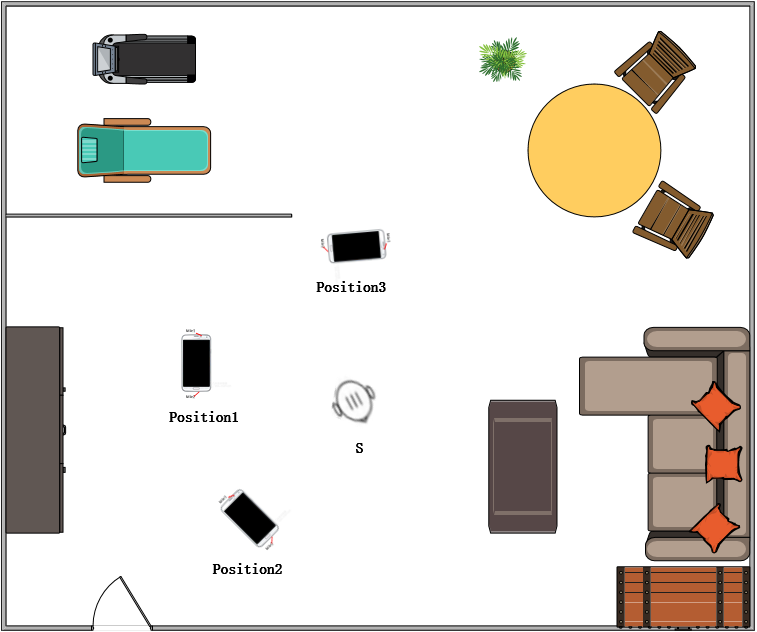
\includegraphics[width=\textwidth]{indoor.png} 
			\caption{{室内环境}}
			\label{fig: indoor}
			%\vspace{0.8cm} % 用来调整和下方文字的间距
		\end{figure}
		
		TODO
		Chan算法简述
		精度数据下一章说明
	
	\section{offline到online的迁移}
	
		\subsection{概念阐述}
			
			offline处理流程尽管可以获得更为精确的结果,但是在实际操作中过于复杂,并且在实际寻找的过程中,我们也并不是“视而不见”,简单的提示信息或许就可以帮助我们的进行探测,因此我们降低了实际需求,从精确到3D指引降至2.5D的探测范围。因此在offline算法的处理的基础上,我们提出了online的处理流程。
		
			这里我们需要更新之前的处理流程,因为在online的处理流程中,麦克风处于一直的录音状态,因此有效声音提取部分也就不是那么重要,在前面的讲解中,我们指出无效声音段并不是声音信号的主体,因此可以直接抛弃一些数据。尽管online的处理流程也可以看做多个offline的组成,但是在实际操作中,我们还是不希望在寻找过程中,在一个位置上长期停留,后续,我们引入一些机制进行一些状态的判断。
			
			首先,我们需要提出一种降维的思想。如图\ref{fig: 3D-dimension-reduction},记智能手机屏幕所在平面为$\text{P}_1$,声源实际位置$\text{S}$与两个麦克风$\text{mic}_1$,$\text{mic}_2$所在平面为$\text{P}_2$,记$\text{P}_1$和$\text{P}_2$构成二面角为$\alpha$,在$\text{P}_2$中,声源位置$\text{S}$与智能手机中心的连线$\text{l}_1$与麦克风所在直线$\text{l}_2$夹角为$\beta$,声源在平面$\text{P}_1$的投影$\text{S}^{'}$与智能手机中心的连线$\text{l}_3$与麦克风所在直线$\text{l}_2$夹角为$\gamma$.显然很容易得到$\tan \gamma = \cos \alpha \cdot \tan \beta$.图中$\text{l}_4$为平面$\text{P}_1$上与麦克风所在直线$\text{l}_2$夹角为$\beta$的直线。尽管$\alpha$的值我们无法获知,但是计算出一个粗略的$\beta$,依然有一定的指导意义,因为在平面$\text{P}_1$上,声源投影的位置$\text{S}^{'}$的方向角$\gamma = \arctan (\cos \alpha \cdot \tan \beta)$。
			
			\begin{figure}[H]
				\centering
				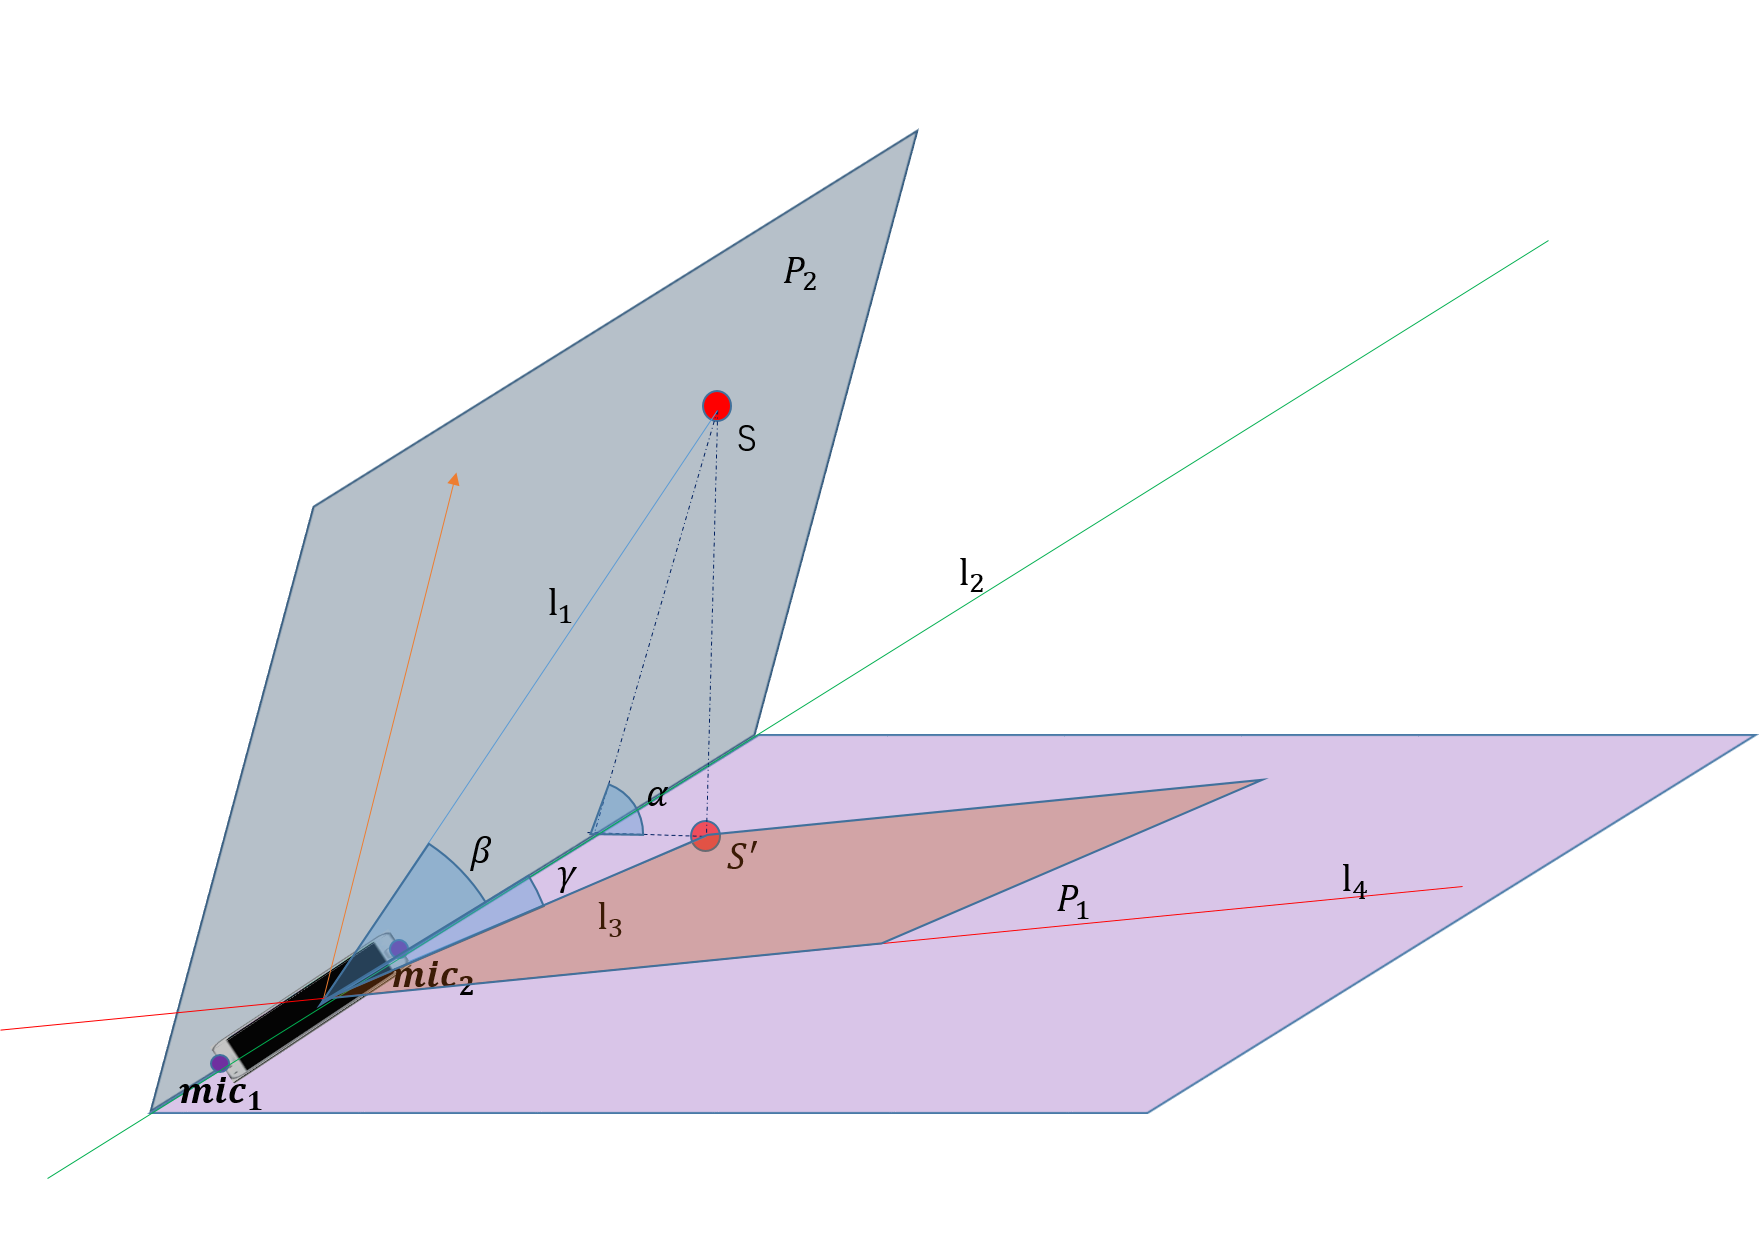
\includegraphics[width=\textwidth]{3D-dimension-reduction.png} 
				\caption{{3D降维指引}}
				\label{fig: 3D-dimension-reduction}
				%\vspace{0.8cm} % 用来调整和下方文字的间距
			\end{figure}
			
			如果在平面$\text{P}_1$上仍使用$\beta$作为指引的方向,那么,这里就会产生一个角度上偏离误差$\delta \theta = \beta - \arctan (\cos \alpha \cdot \tan \beta)$,显然当$\alpha$越大时,误差$\delta \theta$越大(这里$\alpha$不超过90度)。显然在实际运行过程中,我们并不需要考虑这种情况。这是因为实际过程中,智能手机并非是固定不动的,因此,稍微的转动就可以使得二面角发生较大的变化。如图\ref{fig: 3D-dimension-reduction2}所示,当手机位于$\text{Loc}_1$时,二面角$\alpha$达到90度,但是只要稍微转动至$\text{Loc}_2$处,就可以获得一个新的$\alpha$,甚至我们可以把手机移动到$\text{Loc}_3$处。当手机的转动已经不能造成二面角$\alpha$较大的变化时,我们也就来到了声源投影位置的附近区域,这样,声源的位置我们也就大致获得了。
			
			\begin{figure}[H]
				\centering
				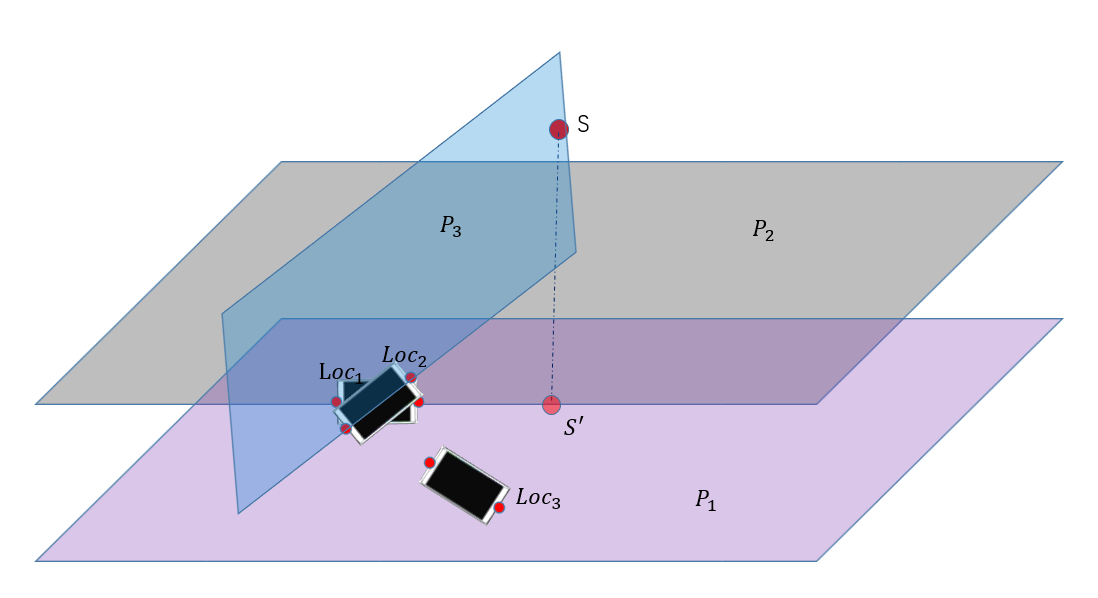
\includegraphics[width=\textwidth]{3D-dimension-reduction2.png} 
				\caption{{手机状态改变}}
				\label{fig: 3D-dimension-reduction2}
				%\vspace{0.8cm} % 用来调整和下方文字的间距
			\end{figure}	
		
		\subsection{online算法模型}
		
	
\chapter{模型系统实现与实验分析}
	\section{开发环境与平台}
	\section{系统设计}
		\subsection{多模块设计}
		\subsection{界面与运行方式}
	\section{实验与分析}
	\section{本章小结}
%%%%%%%%%%%%%%%%%%%%%%%%%%%%%%%%%%%%%%%%%%%%%%%%%%%%%%%%%%%%%%%%%%%%%%%%%%%%%%%
\chapter{总结与展望}
	\section{工作总结}
	\section{前景展望}
%%%%%%%%%%%%%%%%%%%%%%%%%%%%%%%%%%%%%%%%%%%%%%%%%%%%%%%%%%%%%%%%%%%%%%%%%%%%%%%
\bibliography{sample}
%%%%%%%%%%%%%%%%%%%%%%%%%%%%%%%%%%%%%%%%%%%%%%%%%%%%%%%%%%%%%%%%%%%%%%%%%%%%%%%
	% 致谢
	\begin{acknowledgement}
		
		非常感谢在Dislab实验室度过的两年时光,让我在实验室里拓宽眼界的同时,也不断纠正了自己的学习方法和学习态度。我的毕业论文撰写和系统实现中,也或多或少的遇到许多困难,也走过很多弯路。我很感谢我的导师谢磊副教授,从我毕设选题阶段,到我研究工作的开展,再到最后的论文撰写中,谢老师都给予了我细心的指导和点拨,给我纠正了很多错误的方向,避免我走了很多弯路。在实验室的两年,谢磊老师也给我的研究工作不断指引方向,在此,我向谢磊老师致以最真挚的谢意。
		
		同样,我也要感谢在Dislab实验室的同一课题组的各位师兄师姐,鲁欣然师兄在我的成长道路上指引了很多,从细节方面给予我帮助,王楚豫师兄同样,给了我研究工作上的很多帮助,让我的研究工作变的富有创新,也是他们给我提出的宝贵建议,让我可以不断改进自己。
		
		感谢大学四年来四种相伴的同学和朋友,因为你们的存在,我的大学才会在忙碌中透露出精彩。感谢每一位悉心教导我的老师,感谢钱柱中教授的指引,让我能够去香港游学增长知识和阅历,让我在问题求解的课程中感受到计算机和算法的魅力。
		
	\end{acknowledgement}
%%%%%%%%%%%%%%%%%%%%%%%%%%%%%%%%%%%%%%%%%%%%%%%%%%%%%%%%%%%%%%%%%%%%%%%%%%%%%%%
\end{document}
